\chapter{Principes des algorithmes utilisés}
\section{Apprentissage par renforcement}
L'apprentissage par renforcement est une technique d'\textbf{apprentissage automatique} où un agent doit apprendre à maximiser la récompense qu'il reçoit au sein d'un environnement. L'agent a accès à un modèle de l'environnement duquel il observe les différents états et les récompenses associées aux transitions entre ces derniers. Afin de maximiser la récompense obtenue, l'agent peut effectuer des actions, et il devra donc apprendre laquelle est la plus propice à le mener à une récompense importante selon l'état où il se trouve.
\par
Il est commun pour l'apprentissage par renforcement de se baser sur le \textbf{Processus de Décision Markovien} (PDM). Un processus de décision markovien décrit un problème (dans notre cas, en temps discret), avec des ensembles d'états $s$ et d'actions $a$ (dans notre cas, finis), ainsi qu'une fonction de récompense $R_a(s,s')$ fournissant la récompense associée en passant de l'état $s$ à $s'$ en effectuant l'action $a$. L'état résultant d'une action effectuée par l'agent est (en général) en partie aléatoire ou imprévisible.
\par
L'agent doit à partir de toutes ces informations aboutir à une \textbf{politique}, qui lui permettra de choisir la meilleure action dans un contexte donné (celle qui lui permettra de maximiser les récompenses obtenues sur le long terme).
\par

\section{Q-Learning}
\subsection{Principe}
Le Q-Learning est une technique d'apprentissage par renforcement où pour chaque action $a$ possible dans l'état $s$, une fonction $Q(s,a)$ représente la "qualité" de l'action dans le contexte de cet état.
\par
En pratique, on utilisera un tableau en deux dimensions dont une dimension contient les actions possibles, et l'autre les états possibles, ces tableaux sont parfois appelés "Q-Table". Dans ce tableau, chaque cellule située à l'intersection de la colonne d'action $a$ et la ligne d'état $s$ représente la valeur de $Q(s,a)$, les cellules sont initialisées avec pour valeur 0 (en général, cette valeur est arbitraire).

\begin{figure}
\centering
\begin{tabular}{| c | c | c | c | c |}
    \hline
    & Action 1 & Action 2 & $\cdots$ & Action n\\ \hline
    Etat 1 & 0 & 0 & & 0 \\ \hline
    Etat 2 & 0 & 0 & & 0 \\ \hline
    $\vdots$ & & & $\ddots$ & \\ \hline
    Etat m & 0 & 0 & & 0 \\ \hline
\end{tabular}
\caption{Structure d'une Q-Table}
\end{figure}


\subsection{Apprentissage}
Au fil de l'exécution de l'algorithme, on met à jour les cellules du tableau jusqu'à avoir des valeurs optimales dans chacune des cellules.
L'algorithme repose essentiellement sur l'équation de Bellman qui permet de mettre à jour une cellule $Q(s,a)$ à l'aide des informations sur l'état obtenu $s'$ en effectuant l'action $a$ à l'état $s$ :
\[
    Q(s,a) = Q(s,a) + \alpha . \left( r + \gamma . \underset{a'}{max}\, Q(s',a') - Q(s,a) \right)
\]
Ici $s$ et $s'$ sont l'état actuel et l'état suivant, $a$ est l'action effectuée pour passer de $s$ à $s'$, et $r$ est la récompense obtenue en arrivant à l'état $s'$. \par

\subsubsection{Facteur d'apprentissage}
$\alpha$ est le \textbf{facteur d'apprentissage} (learning rate), s'il est égal à 0, la cellule n'est jamais mise à jour, s'il est égal à 1, l'ancienne valeur de la cellule est remplacée par 
\[Q(s,a) = r + \gamma . \underset{a'}{max}\, Q(s',a')\]
(on ne garde aucune trace de l'ancienne valeur).
Il est donc commun de faire baisser peu à peu $\alpha$ au fil de l'apprentissage : au début de l'apprentissage, il n'y a aucun intérêt à garder la valeur initiale de $Q(s,a)$ (choisie arbitrairement), et a la fin de l'apprentissage on espère approcher la valeur réelle de $Q(s,a)$, on modifie donc la valeur de la cellule petit à petit.

\subsubsection{Facteur d'actualisation}
$\gamma$ est le \textbf{facteur d'actualisation} (discount factor), il définit l'importance des récompenses ultérieures. S'il est égal à 0, l'agent choisira la meilleure action à chaque état donné, mais ne tiendra pas compte des récompenses qu'il pourrait obtenir sur le long terme. Et on sait grâce aux propriétés mathématiques des PDM que s'il est égal ou supérieur à 1, la valeur des cellules divergera.

\subsubsection{Explication intuitive de la formule}
La formule de $Q(s,a)$ peut aussi s'écrire de cette façon (à noter que cette formule représente en réalité une affectation):
\begin{equation*}
\begin{aligned}
    Q(s,a) &= Q(s,a) + \alpha . \left( r + \gamma . \underset{a'}{max}\, Q(s',a') - Q(s,a) \right) \\
    & = (1 - \alpha) . Q(s,a) + \alpha . \left( r + \gamma . \underset{a'}{max}\, Q(s',a') \right)
\end{aligned}
\end{equation*}

La première partie de l'affectation ($(1 - \alpha) . Q(s,a)$) représente quel pourcentage de l'ancienne valeur de $Q(s,a)$ sera gardée en fonction de la valeur de $\alpha$. \par
La deuxième partie de l'affectation ($\alpha . \left( r + \gamma . \underset{a'}{max}\, Q(s',a') \right)$) contient les valeurs utilisées pour apprendre. $r$ est la récompense de l'action $a$ à l'état $s$, tandis que $\underset{a'}{max}\, Q(s',a')$ est la valeur maximale de $Q$ qu'on peut espérer obtenir à l'état $s'$ (l'état dans lequel l'agent se trouve une fois $a$ effectué sur $s$), c'est donc ce qu'on estime pouvoir obtenir au mieux dans le futur en effectuant l'action $a$. Cette valeur est pondérée par $\gamma$ pour donner une importance plus ou moins grande aux récompenses futures. Enfin, le tout est pondéré par $\alpha$ afin de modifier la vitesse à laquelle l'agent apprend.


\subsection{Limites}
La "Q-Table" utilisée par l'algorithme implique que l'agent ait connaissance de chaque combinaison d'action et d'état possible pour prendre sa décision. Ainsi en réalité l'algorithme ne fait que mémoriser toutes les possibilités et leur résultat afin de prendre la meilleure décision, mais dans le cas où le nombre de combinaisons possibles devient très important, le Q-Learning n'est plus adapté. \par
Si le problème de la taille du tableau à stocker qui grandit très vite n'est pas négligeable, c'est surtout le problème de temps d'exploration nécessaire pour arrivée à une Q-Table "complète" et stable qui pose problème.

\begin{figure}
    \centering
    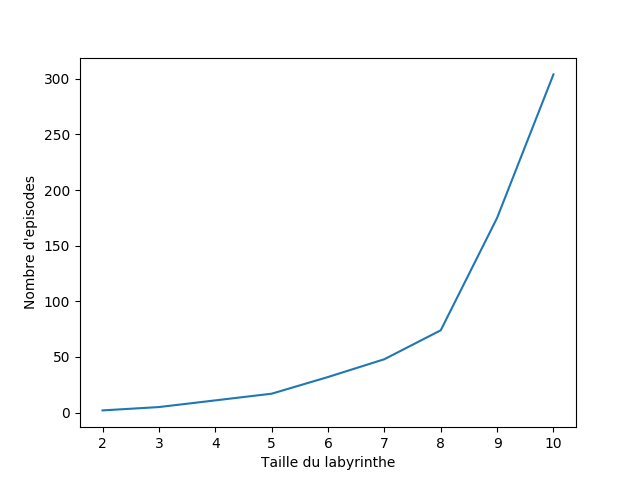
\includegraphics[width=0.7\textwidth]{images/graph_ep_maze.png}
    \caption{Évolution du nombre d'épisodes nécessaires pour arriver au nombre minimal d'étapes dans un labyrinthe de taille donnée (un labyrinthe de taille $x$ contient $x^2$ états)}
\end{figure}

\par
Il est aussi intéressant de noter que cet algorithme ne permet pas de gérer les environnements dont les états sont représentés à l'aide de réels (le nombre d'états n'est alors pas discret), et que ce genre d'environnement est relativement commun.


\section{Apprentissage profond (Deep Learning)}
\subsection{Motivations}
Le problème principal du Q-Learning est son incapacité à déduire un comportement lorsqu'il se trouve dans un état inconnu, en conséquence son fonctionnement est basé sur la mémorisation exhaustive.
Le Deep Learning permet quant à lui à la fois de mémoriser et de déduire à partir de valeurs inconnues, il semble donc intéressant de se pencher sur cette méthode d'apprentissage qui semble pallier les problèmes rencontrés jusqu'ici.

\subsection{Réseau de neurones artificiels}
\subsubsection{Neurone artificiel}
Un neurone artificiel est une fonction à $n$ entrées $\mathbf{x}$ et une seule sortie $y$. Chaque neurone dispose d'une liste de $n$ poids $\mathbf{w}$ (autant que d'entrées), d'un biais $b$, et d'une fonction d'activation $g$. Pour calculer la sortie d'un neurone, il suffit d'effectuer la somme pondérée des entrées $h$ à laquelle on ajoute le biais, puis de calculer la fonction d'activation avec $h$ comme paramètre.

\begin{equation*}
\begin{aligned}
    h &= \sum_{i=1}^{n}(x_i . w_i) + b \\
    y &= g(h)
\end{aligned}{}
\end{equation*}



\begin{figure}
    \centering
    \begin{tikzpicture}[
        init/.style={
          draw,
          circle,
          inner sep=2pt,
          font=\Huge,
          join = by -latex
        },
        squa/.style={
          draw,
          inner sep=2pt,
          font=\Large,
          join = by -latex
        },
        start chain=2,node distance=13mm
        ]
        \node[on chain=2] 
          (x2) {$x_2$};
        \node[on chain=2,join=by o-latex] 
          {$w_2$};
        \node[on chain=2,init] (sigma) 
          {$\displaystyle\Sigma$};
        \node[on chain=2,squa,label=above:{\parbox{2cm}{\centering Fonction \\ d'activation}}]   
          {$g$};
        \node[on chain=2,label=above:Sortie,join=by -latex] 
          {$y$};
        \begin{scope}[start chain=1]
        \node[on chain=1] at (0,1.5cm) 
          (x1) {$x_1$};
        \node[on chain=1,join=by o-latex] 
          (w1) {$w_1$};
        \end{scope}
        
        \begin{scope}[start chain=3]
        \node[on chain=3] at (0,-1.5cm) 
          (x3) {$x_3$};
        \node[on chain=3,label=below:Poids,join=by o-latex] 
          (w3) {$w_3$};
        \end{scope}
        
        \node[label=above:\parbox{2cm}{\centering Biais \\ $b$}] at (sigma|-w1) (b) {};
        
        \draw[-latex] (w1) -- (sigma);
        \draw[-latex] (w3) -- (sigma);
        \draw[o-latex] (b) -- (sigma);
        
        \draw[decorate,decoration={brace,mirror}] (x1.north west) -- node[left=10pt] {Entrées} (x3.south west);
    \end{tikzpicture}
    
    \caption{Schéma d'un neurone artificiel}
\end{figure}{}




\subsubsection{Réseau de neurones}
Les réseaux de neurones artificiels ont été créés en prenant pour inspiration le fonctionnement d'un cerveau, où des enchaînements de neurones émergent des comportements complexes et capables d'apprentissage.
Depuis peu, les réseaux de neurones artificiels connaissent une montée en popularité grâce à des avancées majeures les rendant de plus en plus efficaces, de plus en plus facilement.
\par
Il existe plusieurs architectures de réseaux de neurones artificiels destinés à des usages plus ou moins complexes et spécifiques. Dans notre cas, nous nous cantonneront à l'utilisation de réseaux de neurones à propagation avant (Feedforward Networks), qui sont parmi les architectures de réseaux les plus simples. Ce genre de réseau est constitué d'une couche de neurones en entrée (Input Layer), d'une couche de neurones en sortie (Ouput Layer), et d'un nombre arbitraire de couches intermédiaires (Hidden Layers).
\par
Un réseau de neurones n'est en résumé qu'une fonction à $n$ entrées et $m$ sorties. Pour cela, il est constitué d'un Input Layer et d'un Output Layer contenant respectivement $n$ et $m$ paramètres. Dans le cas d'un réseau Feedforward, les valeurs de sortie des neurones de chaque couche sont calculées à l'aide des valeurs de sortie de la couche précédente, jusqu'à arriver à l'Output Layer. Chaque neurone d'une couche utilise en entrée toutes les sorties de la couche précédente, à l'exception de la première couche où le $i$ème neurone reçoit la $i$ème entrée.
\par


\begin{figure}
    \centering
    \begin{tikzpicture}[
        plain/.style={
          draw=none,
          fill=none,
          },
        net/.style={
          matrix of nodes,
          nodes={
            draw,
            circle,
            inner sep=8pt
            },
          nodes in empty cells,
          column sep=2cm,
          row sep=-9pt
          },
        >=latex
        ]
        \matrix[net] (mat)
        {
        |[plain]| \parbox{1.3cm}{\centering Input\\layer} & |[plain]| \parbox{1.3cm}{\centering Hidden\\layer} & |[plain]| \parbox{1.3cm}{\centering Output\\layer} \\
        & |[plain]| \\
        |[plain]| & \\
        & |[plain]| \\
          |[plain]| & |[plain]| \\
        & & \\
          |[plain]| & |[plain]| \\
        & |[plain]| \\
          |[plain]| & \\
        & |[plain]| \\    };
        \foreach \ai [count=\mi ]in {2,4,...,10}
          \draw[<-] (mat-\ai-1) -- node[above] {Input \mi} +(-2cm,0);
        \foreach \ai in {2,4,...,10}
        {\foreach \aii in {3,6,9}
          \draw[->] (mat-\ai-1) -- (mat-\aii-2);
        }
        \foreach \ai in {3,6,9}
          \draw[->] (mat-\ai-2) -- (mat-6-3);
        \draw[->] (mat-6-3) -- node[above] {Output} +(2cm,0);
    \end{tikzpicture}
    \caption{Exemple de réseau de neurones à 5 entrées, avec une couche cachée de 3 neurones, et 1 sortie}
\end{figure}{}




\subsection{Apprentissage d'un réseau de neurones}
Comme évoqué précédemment, l'un des intérêts des réseaux de neurones est leur capacité d'apprentissage. Par apprentissage, on désigne la capacité du réseau à se modifier afin d'arriver à produire une valeur attendue quelque soit l'entrée. Dans le cas d'un réseau Feedforward, les valeurs à modifier sont les poids et les biais de chaque neurone.
Plutôt que de modifier radicalement ces valeurs, celles-ci sont modifiées très légèrement, mais sur un nombre important de données. L'objectif est que de ces entraînements résulte un réseau capable de donner une sortie acceptable quelque soit l'entrée qui lui est fournie, même si le réseau n'a jamais été entraîné sur cette entrée précise.
\par
Il est important de bien choisir l'architecture du réseau ainsi que ses hyperparamètres, c'est majoritairement ces choix qui définiront la qualité de l'apprentissage. 

\subsubsection{Architecture}
Dans le cas d'un réseau Feedforward, choisir l'architecture, c'est choisir le nombre d'Hidden Layers et le nombre de neurones de chacun. Plus le nombre d'Hidden Layer est élevé, plus le réseau représentera le problème de manière complexe, ce qui est désirable si le problème est réellement complexe, mais qui peut freiner l'apprentissage et mener à de l'overfitting (sur-ajustement) si le problème est en réalité simple. Le nombre de neurones est lui aussi lié à la complexité du problème, plus un problème est complexe, plus le nombre de neurones devrait être important. Malgré les recherches actives sur le sujet, il n'existe actuellement aucune règle empirique sur le choix du nombre d'Hidden Layer et de neurones. Lorsqu'il est réalisé par un humain ce choix est souvent basé sur l'expérience. Bien que nous ne l'utiliseront pas dans le cadre du projet, une solution efficace à ce problème est l'utilisation d'algorithme génétique appliqué à l'architecture du réseau.

\subsubsection{Hyperparamètres}
On désigne par hyperparamètres toutes les variables qui influent sur l'apprentissage de l'ensemble du réseau. Les plus importants sont généralement le learning rate $\alpha$ et le facteur d'actualisation $\gamma$.
De même que pour l'architecture du réseau il n'existe pas de valeur parfaite pour chaque hyperparamètre, elles dépendront du type de données que l'on souhaite faire apprendre au réseau. Et bien que ce ne soit pas utilisé dans ce projet, il existe des méthodes pour trouver de bonnes valeurs comme le Grid Search, le Random Search, ou encore la plus compliqué Bayesian Optimisation. Bien que très efficaces, il nous a été impossible d'inclure ces méthodes dans le cadre temporel de cette UE.

\subsubsection{Apprentissage}
Les réseaux de neurones sont typiquement entraînés à l'aide de rétropropagations du gradient, qui consistent à donner un couple $(entree, sortie\_attendue)$, et à calculer à l'aide d'une fonction donnée (la fonction de perte) l'erreur entre la sortie attendue et la sortie que le réseau produit. Cette erreur est ensuite propagée de la couche de sortie jusqu'à la couche d'entrée en modifiant à chaque couche les poids de ses neurones pour tenter de minimiser l'erreur.
Si l'architecture du réseau est adaptée au problème et si les hyperparamètres du réseau sont bien choisis, ce dernier devrait aboutir à une configuration de ses poids permettant de donner (en quelque sorte de ``déduire'') la sortie de façon correcte quelque soit l'entrée.
\par


\subsection{Problèmes d'apprentissage}
\subsubsection{Sur-apprentissage}
La façon la plus simple de rater l'apprentissage est de tomber dans un problème de \textbf{sur-apprentissage} (ou sur-interprétation), le réseau est alors trop adapté aux données qui lui on été fournies à l'entraînement, et se montre très peu performant lorsque testé sur des données neuves. Il existe deux façon principale d'arriver à un réseau en sur-apprentissage.

\par
La première est de simplement fournir des données trop peu variées au réseau, qui fonctionnera alors parfaitement sur ces données, mais qui se retrouvera avec des sorties largement incorrectes une fois de nouvelles données fournies. Pour éviter cet écueil, il est pratique courante de mettre de côté un certain nombre de données qui ne seront utilisées que pour les tests, et d'utiliser le reste (la majorité) pour l'entraînement. De cette façon, on peut évaluer le réseau sur des données qui lui sont inconnues.
\par
La deuxième méthode pour tomber dans le sur-apprentissage est de choisir une architecture de réseau trop complexe pour représenter le problème donné. La représentation interne du réseau sera retrouvera trop complexe pour pouvoir interpréter ``simplement'' les données.

\begin{figure}
    \centering
    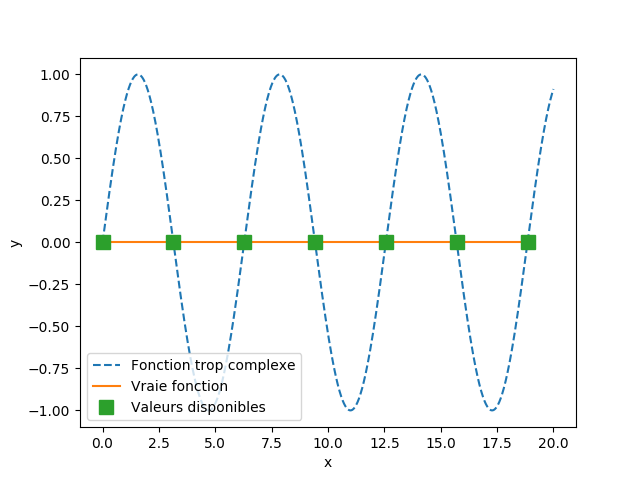
\includegraphics[width=0.7\textwidth]{images/graph_overfitting.png}
    \caption{Voici un exemple d'overfitting : à partir de points tous à y=0, il est possible de déduire une réalité complexe mais fausse (la fonction sin) (la fonction attendue était f(x)=0).}
\end{figure}{}


\subsubsection{Non convergence}
L'objectif lors de l'entraînement d'un réseau, est de converger vers une disposition des poids où l'erreur sur le noeud de sortie est minimale quelque soit l'entrée. Cependant, il est possible de ne jamais parvenir à approcher une erreur faible.
\par
Une cause possible évidente de ce problème est l'architecture du réseau si cette dernière n'est pas assez complexe pour que le réseau puisse modéliser la solution. Par exemple, une propriété connue des réseaux de neurones est qu'il faut au moins 1 Hidden Layer pour que la sortie ne soit pas linéaire (et 2 Hidden Layers suffisent à modéliser n'importe quelle fonction), ce qui veut dire que la fonction XOR est impossible à faire apprendre à un réseau sans Hidden Layer.
\par
Ce problème peut aussi apparaître si les hyperparamètres sont mal choisis. Si on regarde le cas du facteur d'apprentissage $\alpha$ précédemment présenté, on peut déduire qu'un grand nombre de valeurs possibles mèneront difficilement à une solution : s'il est trop grand, l'ancienne valeur de $Q(s,a)$ sera trop vite écrasée et on perd l'aspect "mémorisation" recherché. S'il est trop petit, l'ancienne valeur de $Q(s,a)$ joue une part trop importante et l'apprentissage ne se fait presque pas. De même pour $\gamma$ dont nombre de valeurs rendent l'apprentissage impossible.
\par
Il est donc extrêmement important de choisir l'architecture et les hyperparamètres du réseau en fonction du problème à traiter sous peine de ne pouvoir jamais aboutir à une solution.


\section{Deep Q-Learning (DQN)}
\subsection{Principe}
Comme évoqué précédemment, le Q-Learning possède des défauts que le Deep Learning semble résoudre. Notre objectif est donc de remplacer le Q-Learning par du Deep Learning, et faire ainsi de l'apprentissage par renforcement sur des réseaux de neurones.
Pour cela, nous remplaçons la Q-Table par un réseau de neurones profond. Le rôle de ce réseau est d'approximer la fonction $Q(s,a)$ : le réseau prend en entrée un état $s$ et donne en sortie les $Q(s,a)$ pour chaque action.

\subsection{Fonctionnement}
Le fonctionnement d'un agent utilisant le Q-Learning ou le DQN pour agir dans son environnement est strictement identique : à chaque état $s$, on choisit une action $a$ à l'aide de notre structure de donnée propre (ou en choisissant une action au hasard, selon la politique en vigueur). L'agent utilisant le Q-Learning choisit la case avec la valeur la plus grande de la ligne $s$ de son tableau, tandis que l'agent DQN fournit son état $s$ en entrée du réseau de neurones, et choisit la sortie ayant la plus grande valeur.
\par
Il n'y a donc aucune difficulté apparente de ce côté, les différences majeures se trouvent à l'apprentissage.
Avec le Q-Learning, ce dernier est relativement simple : c'est un processus itératif où les valeurs de la Q-Table sont peu à peu changées pour converger vers une fonction Q(s,a) (dans ce cas représentée par la table) optimale. 
\par
Cependant l'apprentissage d'un réseau de neurones est bien plus complexe, et on remarque dans la partie précédente que la grande difficulté des réseaux de neurones et de réussir à leur faire apprendre une fonction efficacement. Le nombre de problèmes entravant l'apprentissage est significatif.
\par
Pour régler ces problèmes et tirer plein parti du potentiel du Deep Learning, il est nécessaire de mettre en place certaines optimisations. Nous allons donc tenter d'expliciter les plus élémentaires.

\subsection{Experience Replay}
\subsubsection{Approche simpliste}
Avec le Q-Learning, pour savoir comment changer les valeur de sa table, l'agent utilise simplement la transition $(s,a,r,s')$ obtenu après chaque action effectuée ($s$ correspond à un état, $a$ est l'action effectuée à l'état $s$, $r$ est la récompense obtenue suite à l'action $a$ à l'état $s$, et $s'$ est l'état résultat de l'action).
Bien que simple, cette approche est efficace à résoudre les problèmes pour lesquels le Q-Learning est destiné, la convergence vers une solution étant généralement garantie.
\par
Cette approche est en revanche grandement inefficace lorsque appliquée à des réseaux de neurones. Entraîner des réseaux de neurones sur des données successives rend très difficile les chances d'aboutir à un réseau entraîné pour être optimal en tout état. Les chances d'être constamment dans des minimum locaux ou d'être dans une situation d'overfitting adaptée seulement aux données récentes sont bien trop grandes. Ainsi, l'apprentissage s'en retrouve chaotique, instable et inefficace.

\subsubsection{Principe et fonctionnement}
\par
Une solution possible à ces problèmes est la technique de l'\textbf{Experience Replay}, qui consiste à stocker chaque transition $(s,a,r,s')$ dans un buffer, puis à piocher aléatoirement un nombre arbitraire de transitions, et d'entraîner le réseau sur chacune d'entre elles.
\par
En pratique, on utilisera une file de taille fixe afin que les transitions les plus récentes remplacent les plus vieilles. La taille d'Experience Replay la plus populaire est actuellement $10^6$, mais certains papiers soulignent l'importance de bien choisir cet hyperparamètre qui a un impact important sur l'apprentissage \cite{exp_replay_deeper}.
\par
L'algorithme classique d'apprentissage par renforcement avec Experience Replay est donné plus bas.

\begin{algorithm}
\SetAlgoLined

Initialiser l'Experience Replay $M$\\
\Tq {l'apprentissage n'est pas terminé}
{
Placer l'agent dans un état initial\\
\Tq{l'agent n'est pas dans un état terminal}
{
Sélectionner une action $a$ à effectuer d'après la politique actuelle \\
Appliquer l'action $a$ \\
Observer le nouvel état $s'$ et récupérer la récompense $r$\\
Ajouter la transition $(s,a,r,s')$ à $M$\\
Sélectionner un échantillon aléatoire $B$ dans $M$\\
Faire apprendre au réseau d'après chaque transition de $B$
}
}

\caption{Algorithme classique d'apprentissage utilisant l'Experience Replay}
\end{algorithm}

A chaque ``étape'' ou ``pas'' de l'environnement observé (chaque action effectuée), l'agent choisit une action et l'applique,  mémorise la transition résultante, puis entraîne le réseau sur un échantillon de l'Experience Replay $B$. Cet échantillon est communément appelé \textbf{minibatch}.


\subsubsection{Conséquences}
L'utilisation de l'Experience Replay permet d'enlever tout lien de causalité entre chaque action et de permettre au réseau un apprentissage bien plus général du problème. Cela permet aussi de ne pas apprendre des transitions dépendant exclusivement de la politique actuelle de l'agent, on peut par exemple trouver dans l'Experience Replay des transitions effectuées lorsque l'agent avait son hyperparamètre $\epsilon$ égal à 1 alors que sa valeur actuelle est bien plus basse. On en déduit par la même occasion que grâce à l'Experience Replay, le réseau est susceptible d'apprendre plusieurs fois une même transition (à des instants différents) \cite{atari_drl}.
\par
Toutes ces propriétés de l'Experience Replay permettent de contourner les problèmes précédemment évoqués, et bien que cette méthode soit globalement assez efficace pour permettre un bon apprentissage dans les problèmes que nous traitons, l'Experience Replay implique un défaut majeur : l'apprentissage des transitions nouvellement effectuées (potentiellement très cruciales à l'apprentissage) ne se fait pas instantanément, il faut avoir la ``chance'' que l'agent tombe dessus lors de la pioche aléatoire de transitions. Bien que des améliorations du principe ont été créées (Prioritized Experience Replay), à la date de création de ce rapport il semble qu'aucune alternative majeure à l'Experience Replay n'existe.

\subsection{Standardisation des entrées}
Un réseau de neurones accepte en entrée un certain nombre de réels. Les réels peuvent être de n'importe quelle valeur, en théorie cela ne devrait pas poser de problème au réseau : en cas de problème et avec un nombre suffisant d'Hidden Layers, le réseau pourra ``redimensionner'' ces valeurs de façon à contrer la disproportion de grandeurs.
\par
Par exemple, il est possible qu'un des réels fournis en entrée d'importance moindre soit significativement plus grand qu'un autre réel dont l'importance est majeure : mathématiquement, ce n'est pas ce que l'on désire. On sait que le réseau pourra annuler et renverser ce déséquilibrage au fil de l'apprentissage grâce à ses Hidden Layer.
\par
Toutefois, il est très commun de malgré tout normaliser les entrées, que ce soit pour simplement tous les faire tenir dans un intervalle plus réduit (typiquement $[0;1]$ ou $[-1;1]$ ) en redimensionnant toutes les entrées, ou pour ramener toutes les entrées à des ``importances'' identiques en appliquant un redimensionnement adapté à chaque entrée.
\par
Appliquer ce redimensionnement au préalable (en pré-processing) permet d'éviter de complexifier inutilement l'apprentissage du réseau. De plus, les poids du réseau sont initialisés par des valeurs arbitraires, généralement adaptées à des valeurs d'entrée faibles, redimensionner les entrées du réseau permet d'éviter d'adapter ces valeurs.
\par
Ainsi en pratique on normalisera les entrées dès que c'est possible afin de faciliter et accélérer l'apprentissage \cite{ai_faq}.


\subsection{Dropout}
Bien qu'elle soit moins essentielle en reinforcement learning où l'on peut obtenir un nombre quasi infini d'informations pour entraîner le réseau de neurones, la méthode de \textbf{Dropout} (ou ``Abandon'') est un moyen très simple et efficace de réduire le surajustement du réseau.
\par
Son principe est extrêmement simple : lors de l'entraînement, chaque neurone a une chance $p$ d'être ``désactivé'' sa valeur de sortie est alors 0 (il n'a aucune influence sur le réseau). En revanche lors de phases de test (lorsqu'un utilise le réseau), tous les neurones se comportent normalement.

\begin{figure}
    \centering
    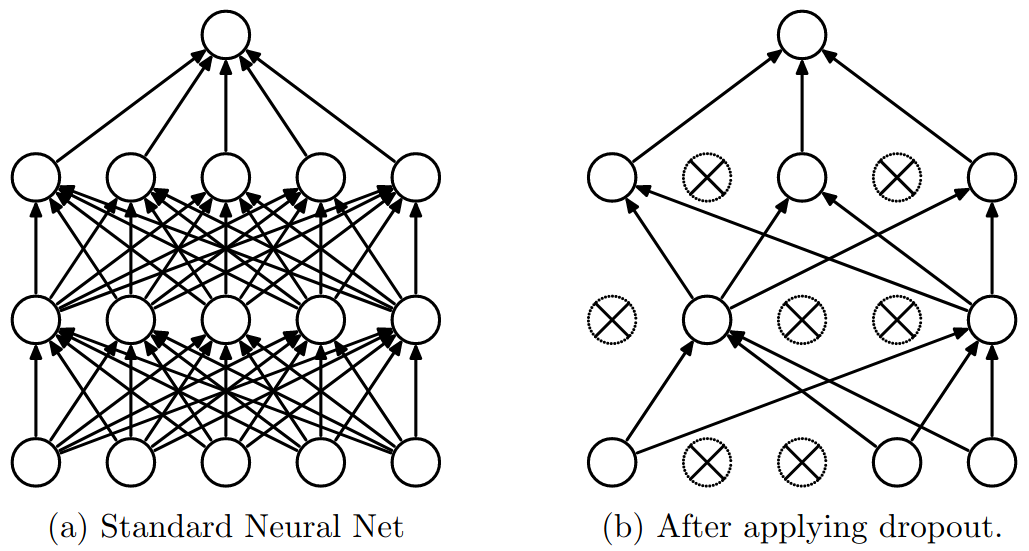
\includegraphics[width=1\textwidth]{images/dropout.png}
    \caption{\textbf{A gauche} (a) : réseaux neuronal standard avec 2 couches cachées. \textbf{A droite} (b) : le même réseau après application du Dropout. Les neurones avec une croix ont été désactivé (drop).
    \\\textit{Schéma tiré du papier original sur le Dropout} \cite{dropout}}
\end{figure}

\par
Il est assez intuitif de comprendre le fonctionnement de cette technique : le réseau évitera de faire de mauvaises ``conjecture'' parce que par coïncidence des neurones s'activent en même temps. Au fil de l'entraînement, on n'entraîne que certaines parties du réseau seulement sur une certaine partie des données (les neurones de la couche d'entrée sont eux aussi susceptibles d'être désactivés).
\par
A la fin de l'entraînement, les chances du réseau d'effectuer de mauvaises ``conjectures'' suites à des coïncidences dans ses données et dans son entraînement seront grandement réduites, et le réseau s'en retrouve en conséquence bien plus efficace.
\par
En pratique, la valeur de $p$ la plus utilisée est $0.5$, qui d'après les études menées sur le sujet, correspond à la grande majorité des situations \cite{dropout}. 